\newpage
\section{Projektplanung}
Es wird der Projektstrukturplan mit den einzelnen Arbeitspaketen gezeigt. Ebenfalls wird der Balkenplan, welcher die Zeit für die jeweiligen Arbeitspakete benötigt wird, vorgestellt.
\subsection{Projektstrukturplan}
Die beiden Back-End-Developer sind für die Desktop-Version des Produkts als auch für die Applikation zuständig. Da sie   im Bereich des kabellosen Datentransfers nur wenig Erfahrung haben müssen sie sich während dem Projekt das Nötige Knowhow erarbeiten. Der Front-End-Developer kümmert sich um die GUI für die Desktop-Version und Applikation. Neben der Erstellung der Interfaces hat dieser auch die Aufgabe das Webportal für das Produkt zu erstellen. Um das beste Ergebnis zu erreichen wird das Projektteam interne Tests als auch eine Zielgruppentestung mit Passanten durchführen.\\
%\begin{comment}
\begin{figure}[H]
	\centering
	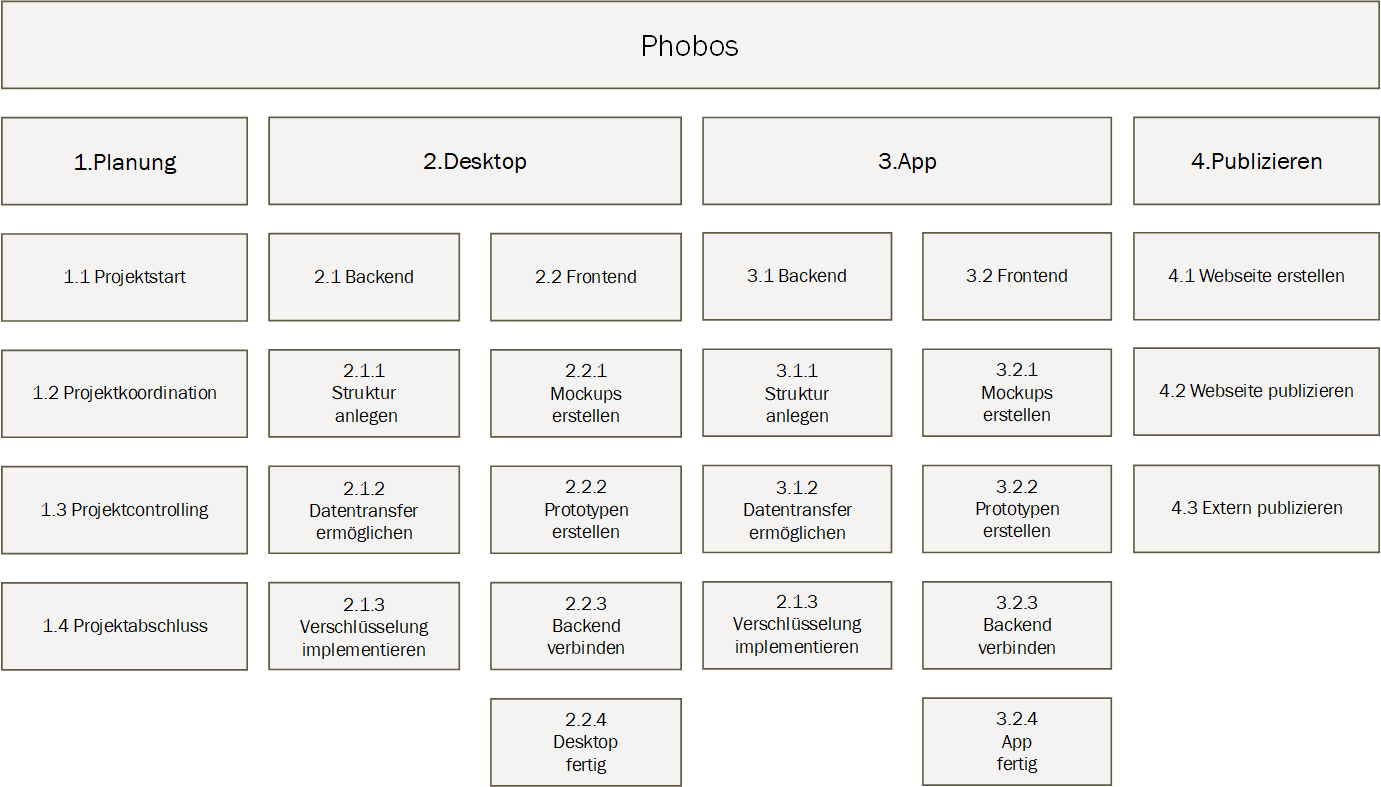
\includegraphics[width=\linewidth]{pictures/8.Projektorganisation/psp.png}\
	\caption{Projektstrukturplan}
\end{figure}
%\end{comment}
\newpage
\subsection{Balkenplan}
Die Arbeitspakete sollen zwischen dem 14.2.2019 und dem 23.05 abgeschlossen werden. Dabei werden 40 Prozent, also ca. 1 Monat, der Zeit für die Projektanfang, Lastenheft, Machbarkeitsstudie und Pflichtenheft, vorgesehen. Der Abschluss von Desktop und App Version werden in dessen Aufwand geplant 55 Prozent der Zeit in Anspruch nehmen. Die Publizierung des Produktes soll die letzten 5 Prozent benötigen.\\
%\begin{comment}
\begin{figure}[H]
\centering
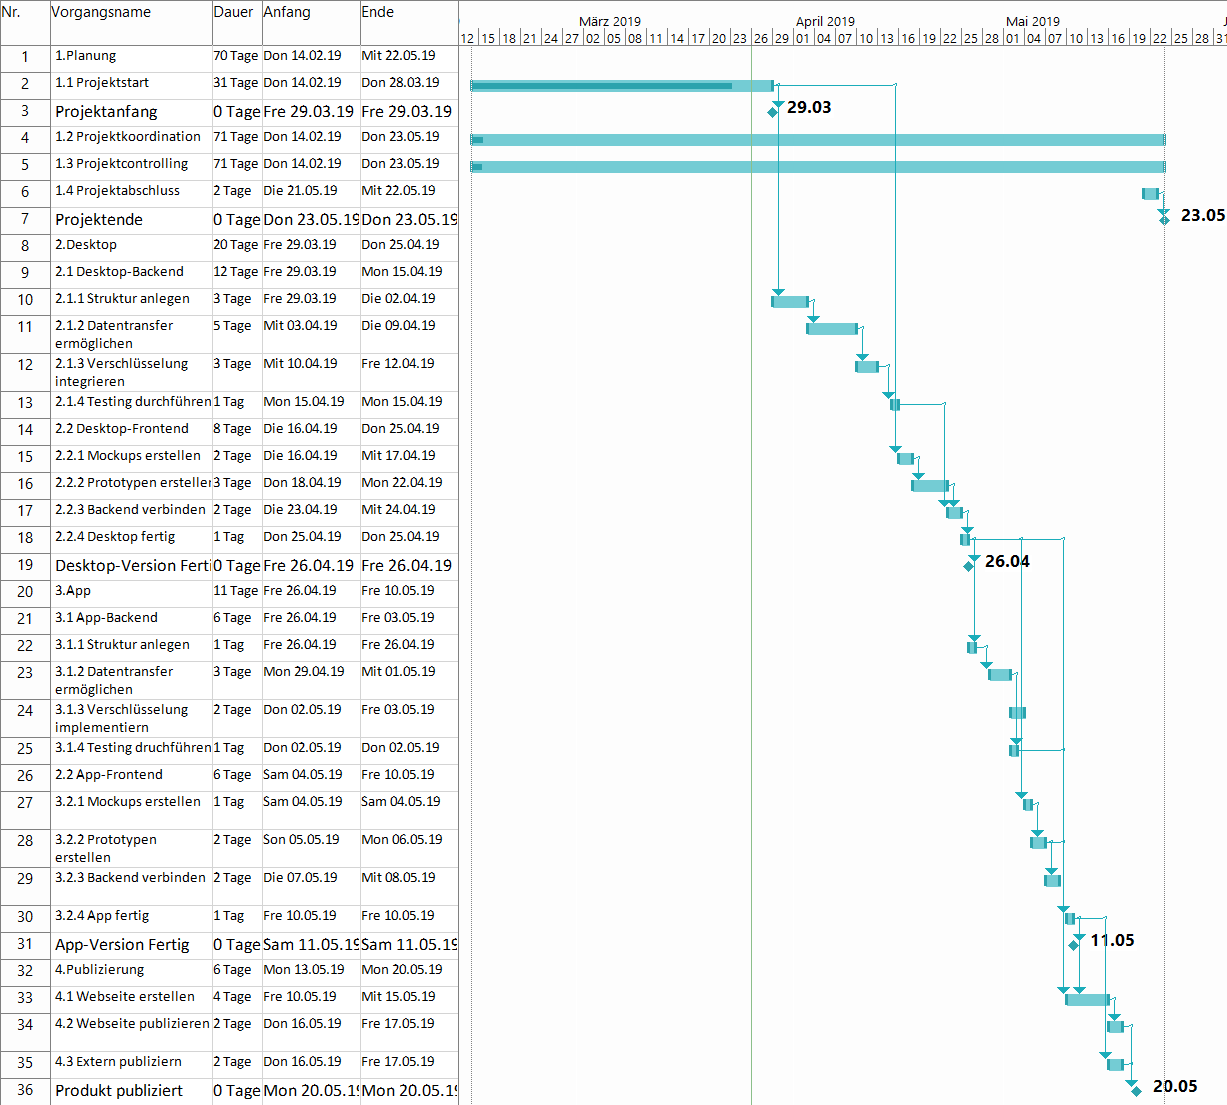
\includegraphics[width=\linewidth]{pictures/8.Projektorganisation/balkenplan.png}\
\caption{Balkenplan}
\end{figure}
%\end{comment}
\newpage
\subsection{Meilensteinplan}
Das Projekt soll voraussichtlich am 23.05.2019 beendet werden. Bis zu diesem Zeitpunkt hat das Projektteam 4 Meilensteine absolviert. Die Beschreibung, was genau bei diesen Meilensteinen abgeschlossen bzw. abgegeben wird, steht in der folgenden Tabelle.
\begin{table}[H]
	\begin{center}
		\begin{tabularx}{\linewidth}{|X|X|X|}
			\hline
			\textbf{Meilenstein}&Deliverable&Datum\\
			\hline
			Projektstart&Alle Dokumente mit den Informationen zum Projekt&Voraussichtlich 29.03.2019\\
			\hline
			Desktop-Version&Funktionsfähige Desktop-Applikation mit allen genannten Funktionen&Voraussichtlich 26.04.2019\\
			\hline
			Smartphone-Version&Funktionsfähige Smartphone-Applikation mit allen genannten Funktionen&Voraussichtlich 11.05.2019\\
			\hline
			Produkt publizieren&Funktionsfähige Webseite mit allen genannten Funktionen. Veröffentlichtes Produkt auf Google Play Store&Voraussichtlich 20.05.2019\\
			\hline
			Projektende&Fertiges Produkt wie vereinbart&Voraussichtlich 23.05.2019\\
			\hline
		\end{tabularx}
	\end{center}
\end{table}